\Exhibit{Diploma1}{Диплом бакалавра Алексея Инкина\WithTr}

Алексей Инкин получил образование бакалавра в Нижегородском Государственном Техническом университете,
выпустившись с отличием в 2006.

Его специалность -- `Информационные системы'.

Нижегородский Государственный Технический университет -- второй крупнейший университет в Нижнем Новгороде (Россия).
Он основан в 1898 году.
Там учатся 13 тысяч студентов, и больше 1000 человек занимаются там наукой и преподают.
Он сотрудничает с университетами, предприятиями и научными организациями в более чем 40 странах
\ExhibitRef{NntuHome}.

\includepdf[pages=-]{diploma_eng_public}

\begin{center}
    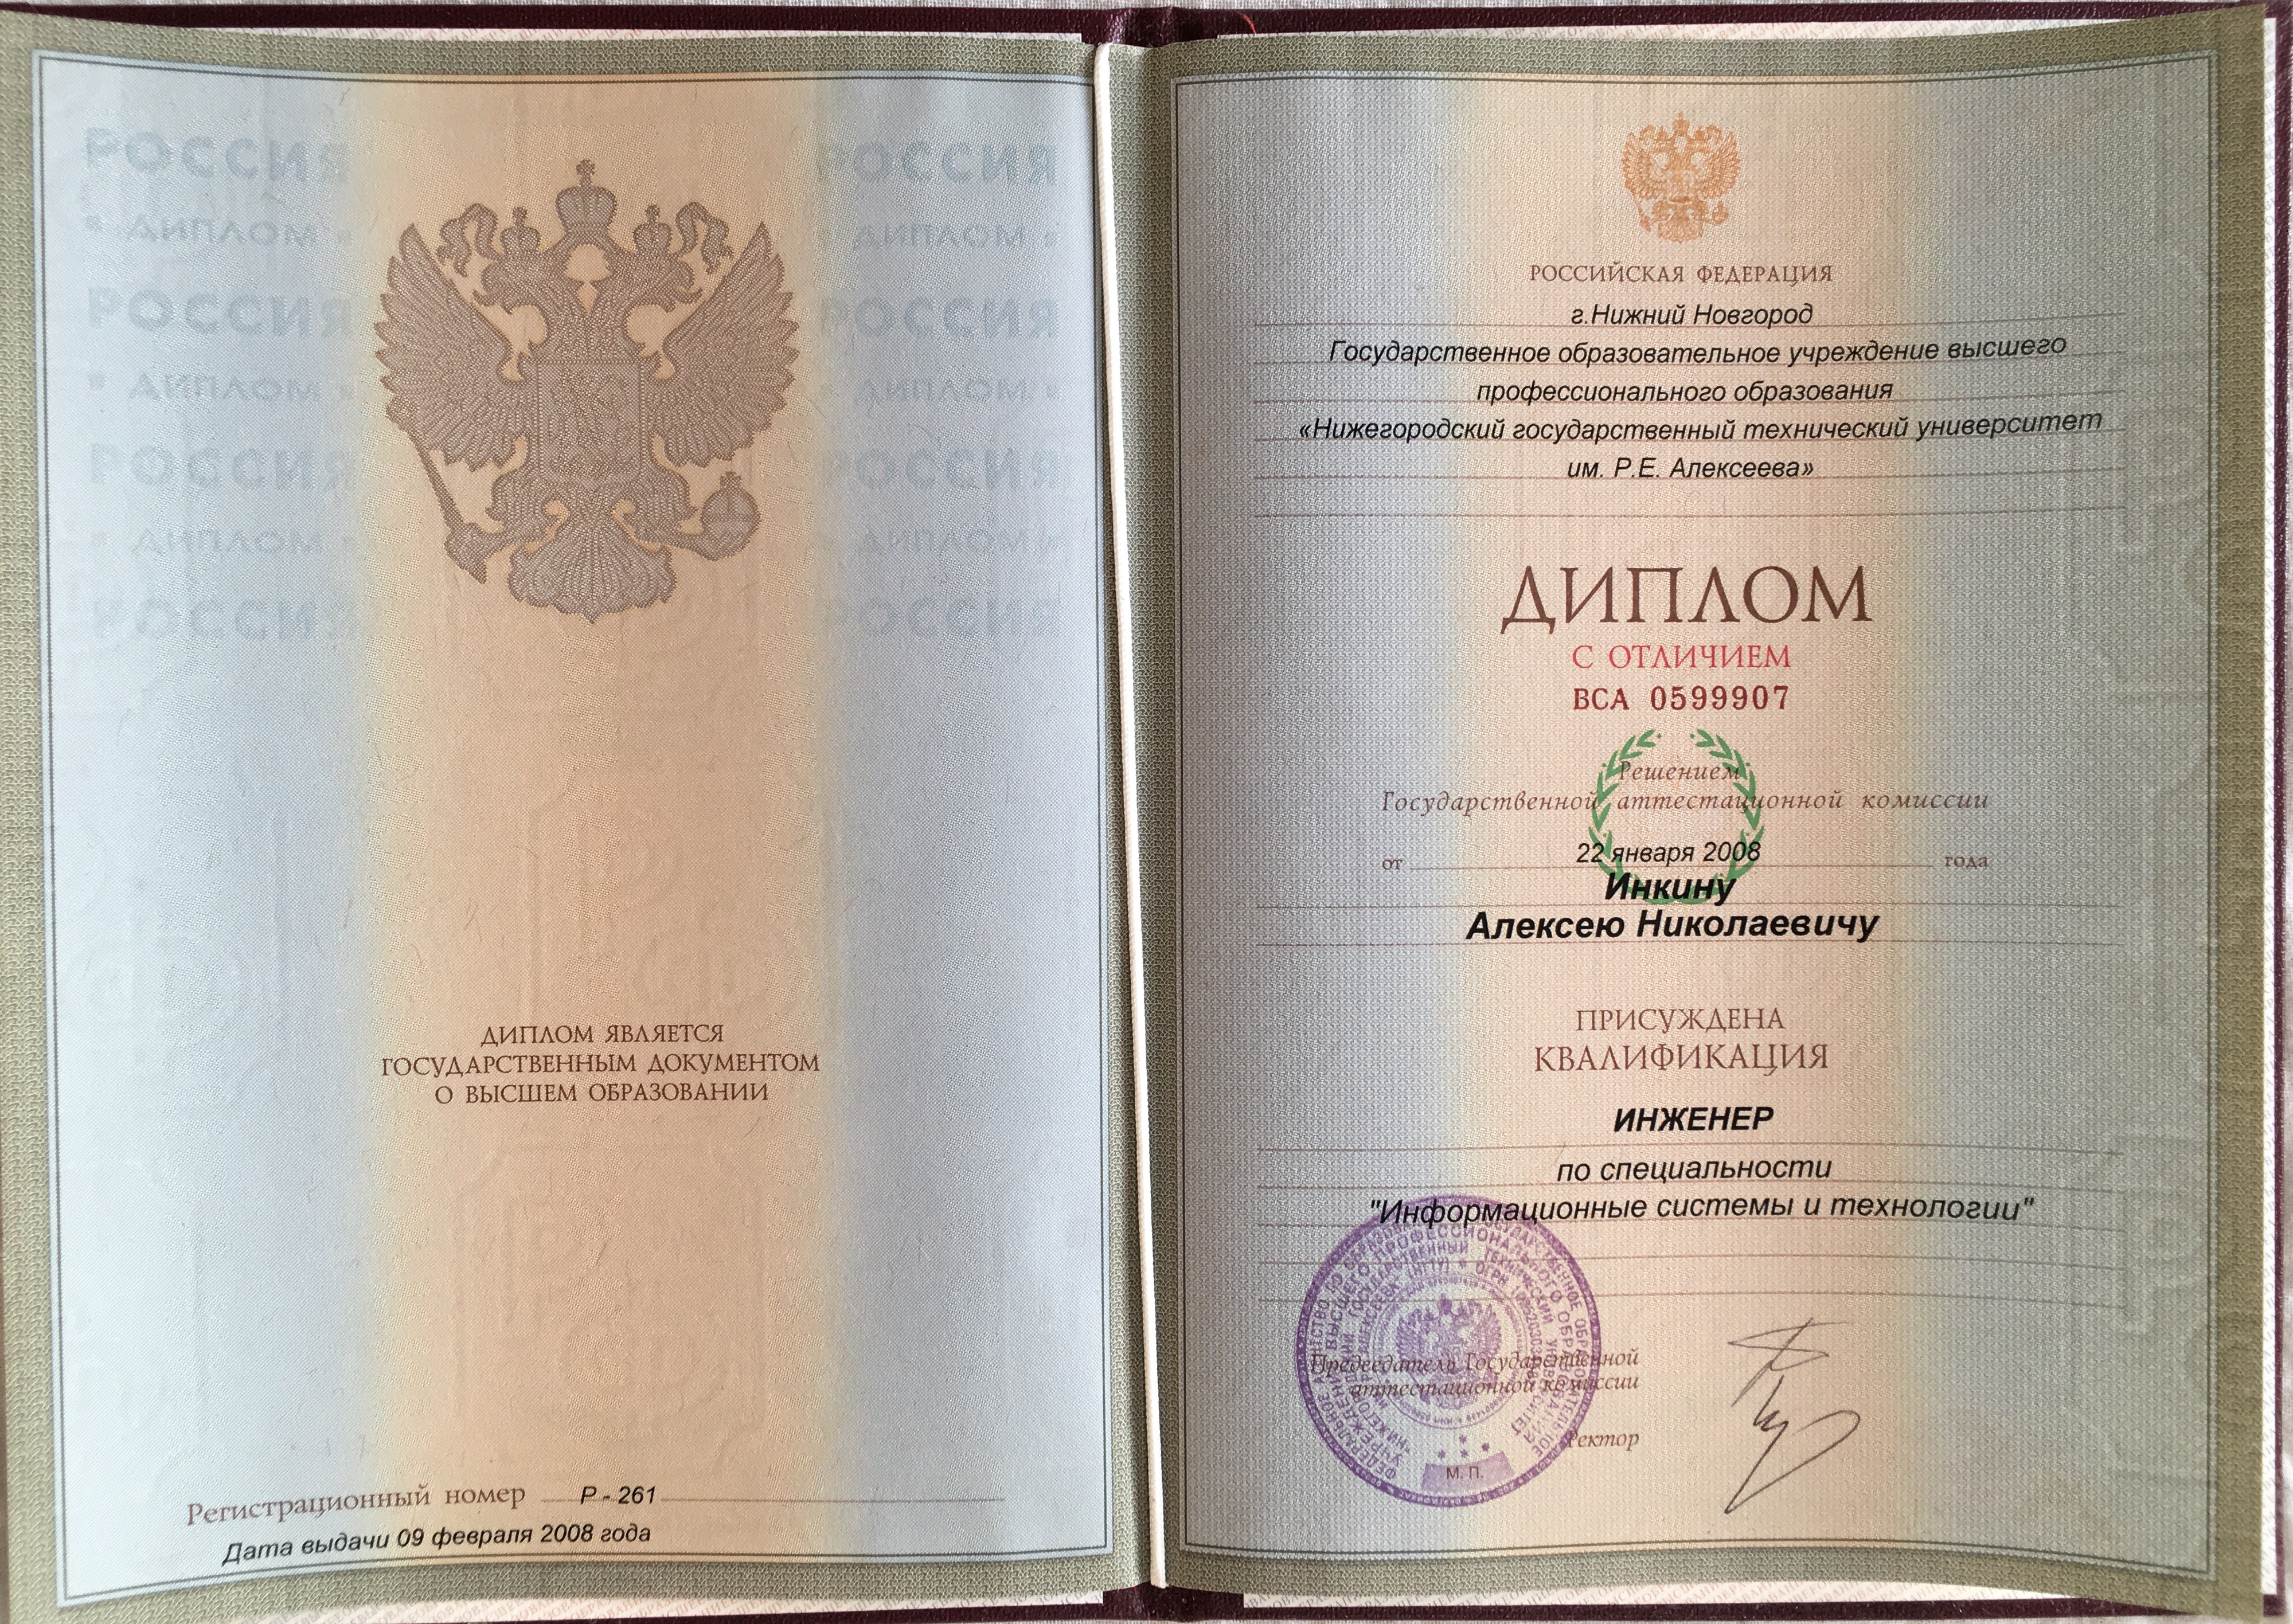
\includegraphics[width=57em,angle=90]{title}
\end{center}
\pagebreak

\begin{center}
    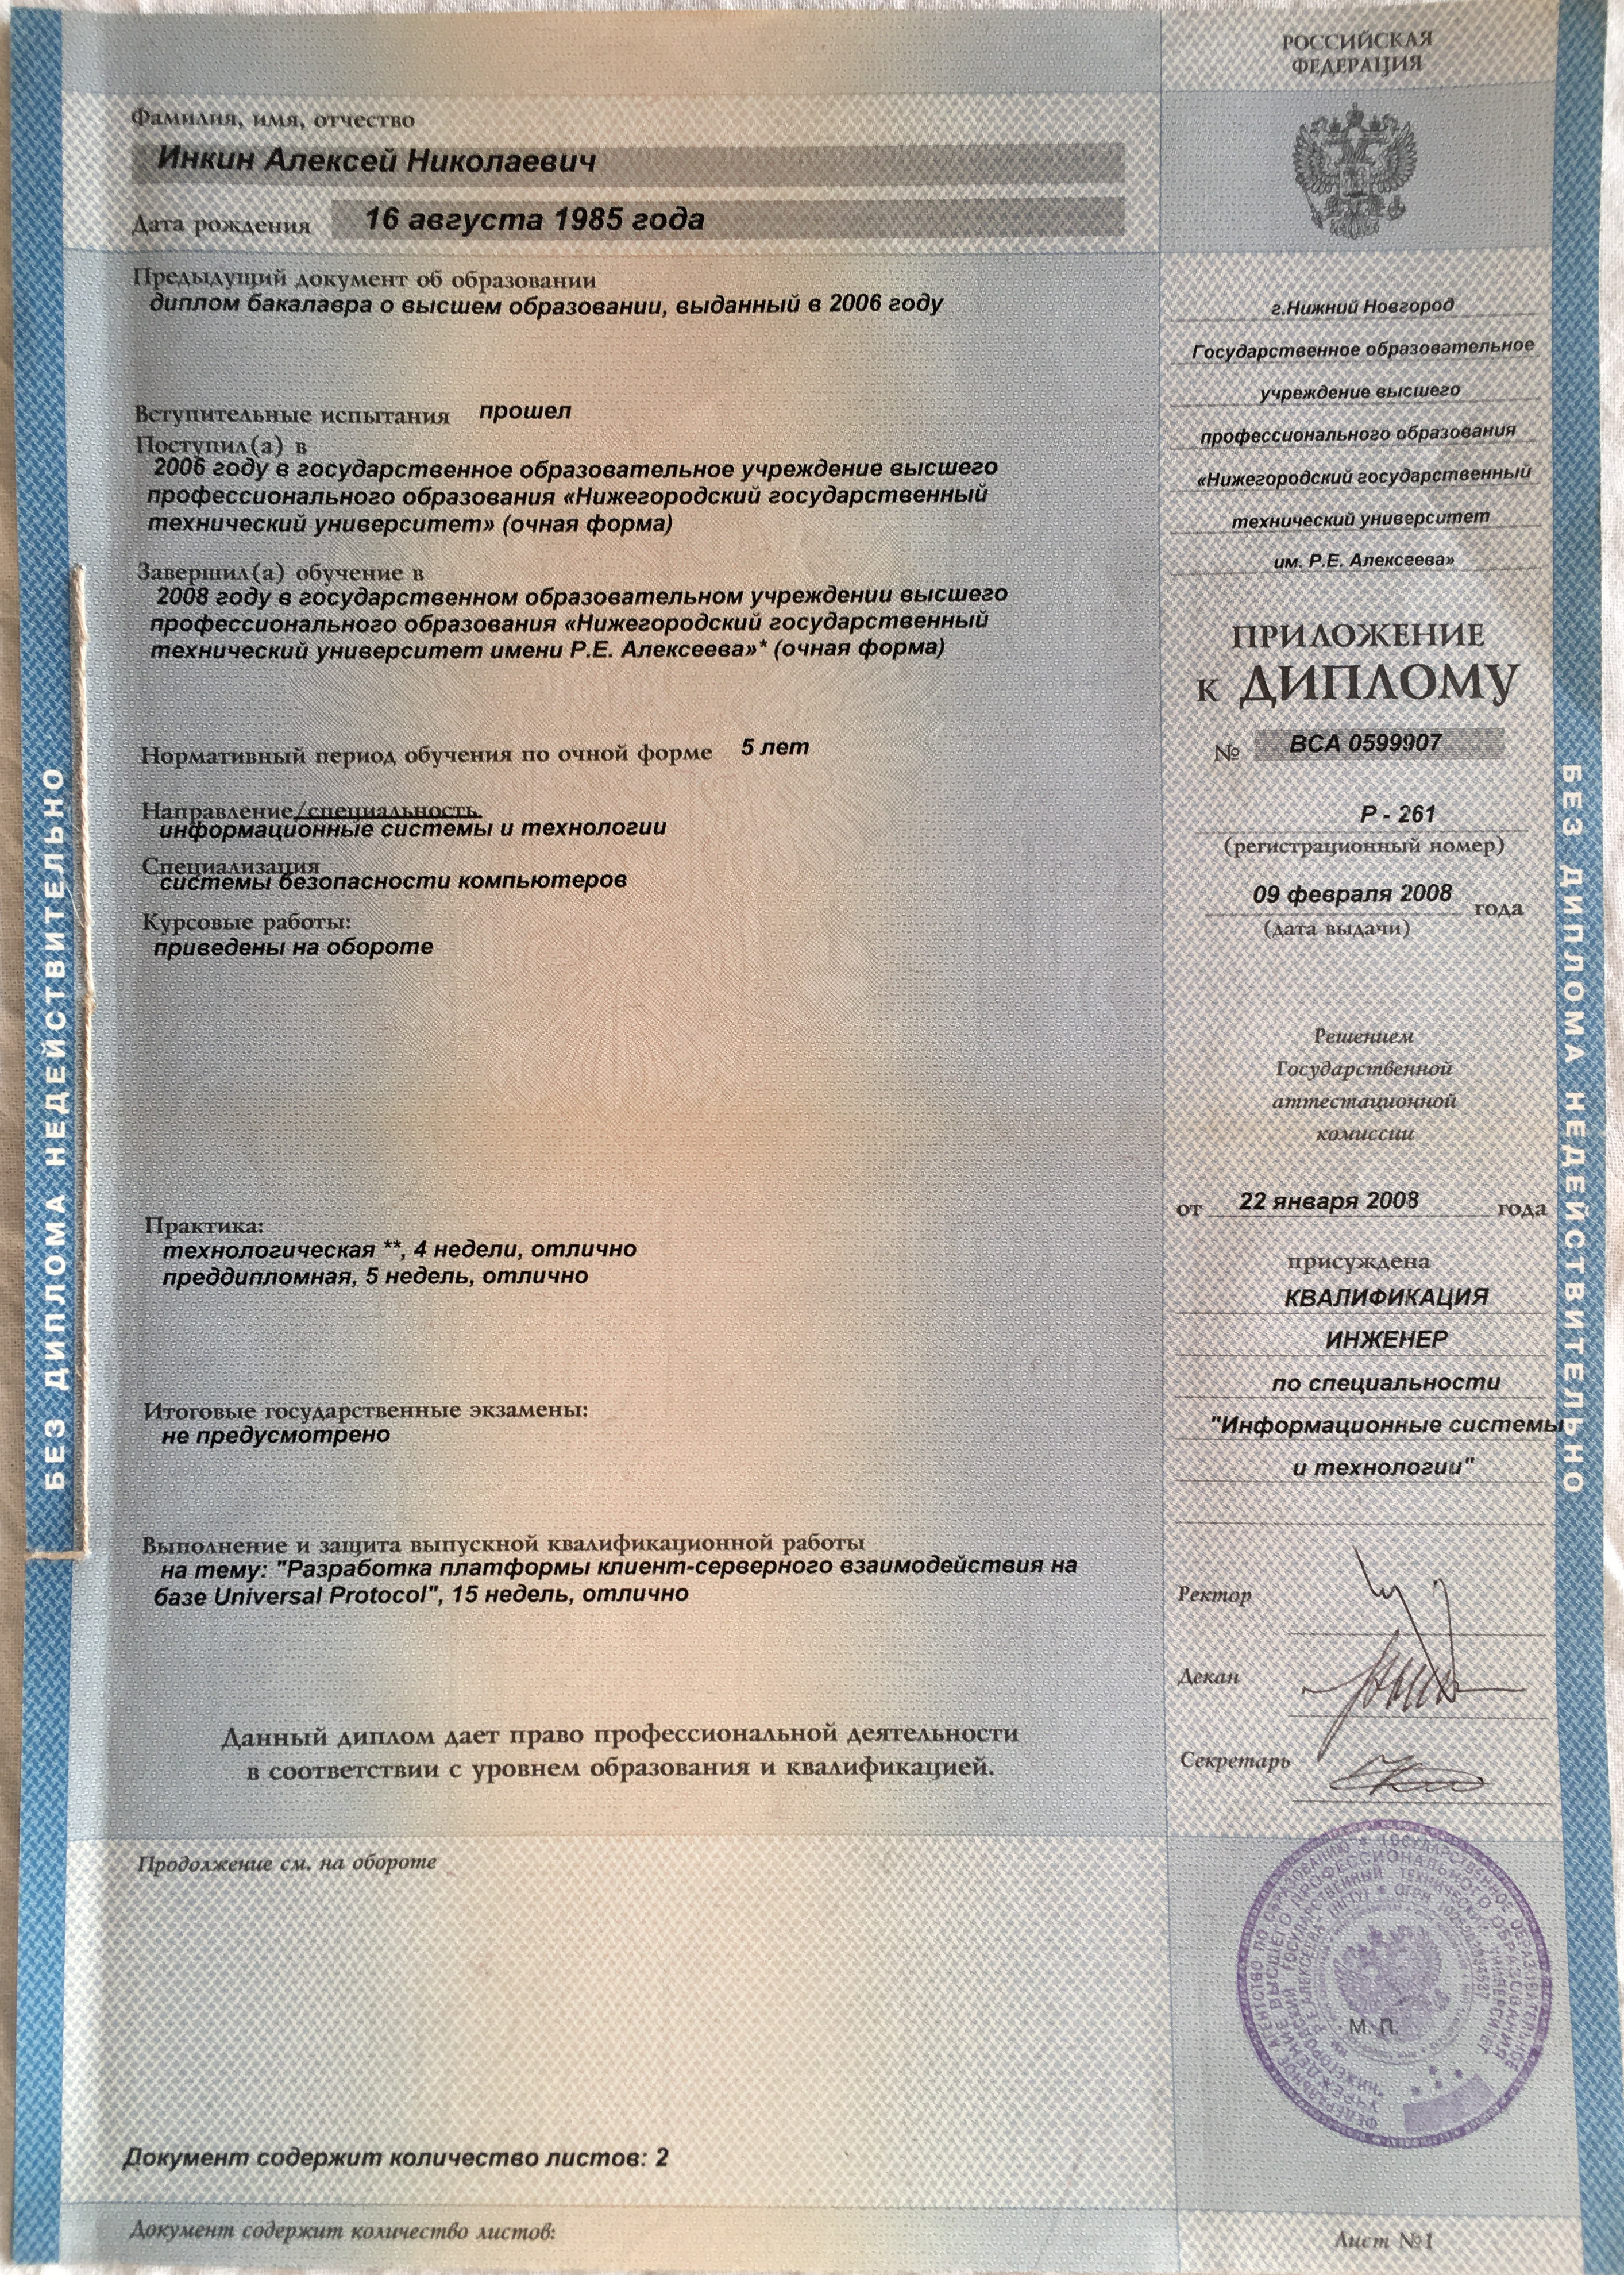
\includegraphics[width=41em]{appendix-1}
\end{center}
\pagebreak

\begin{center}
    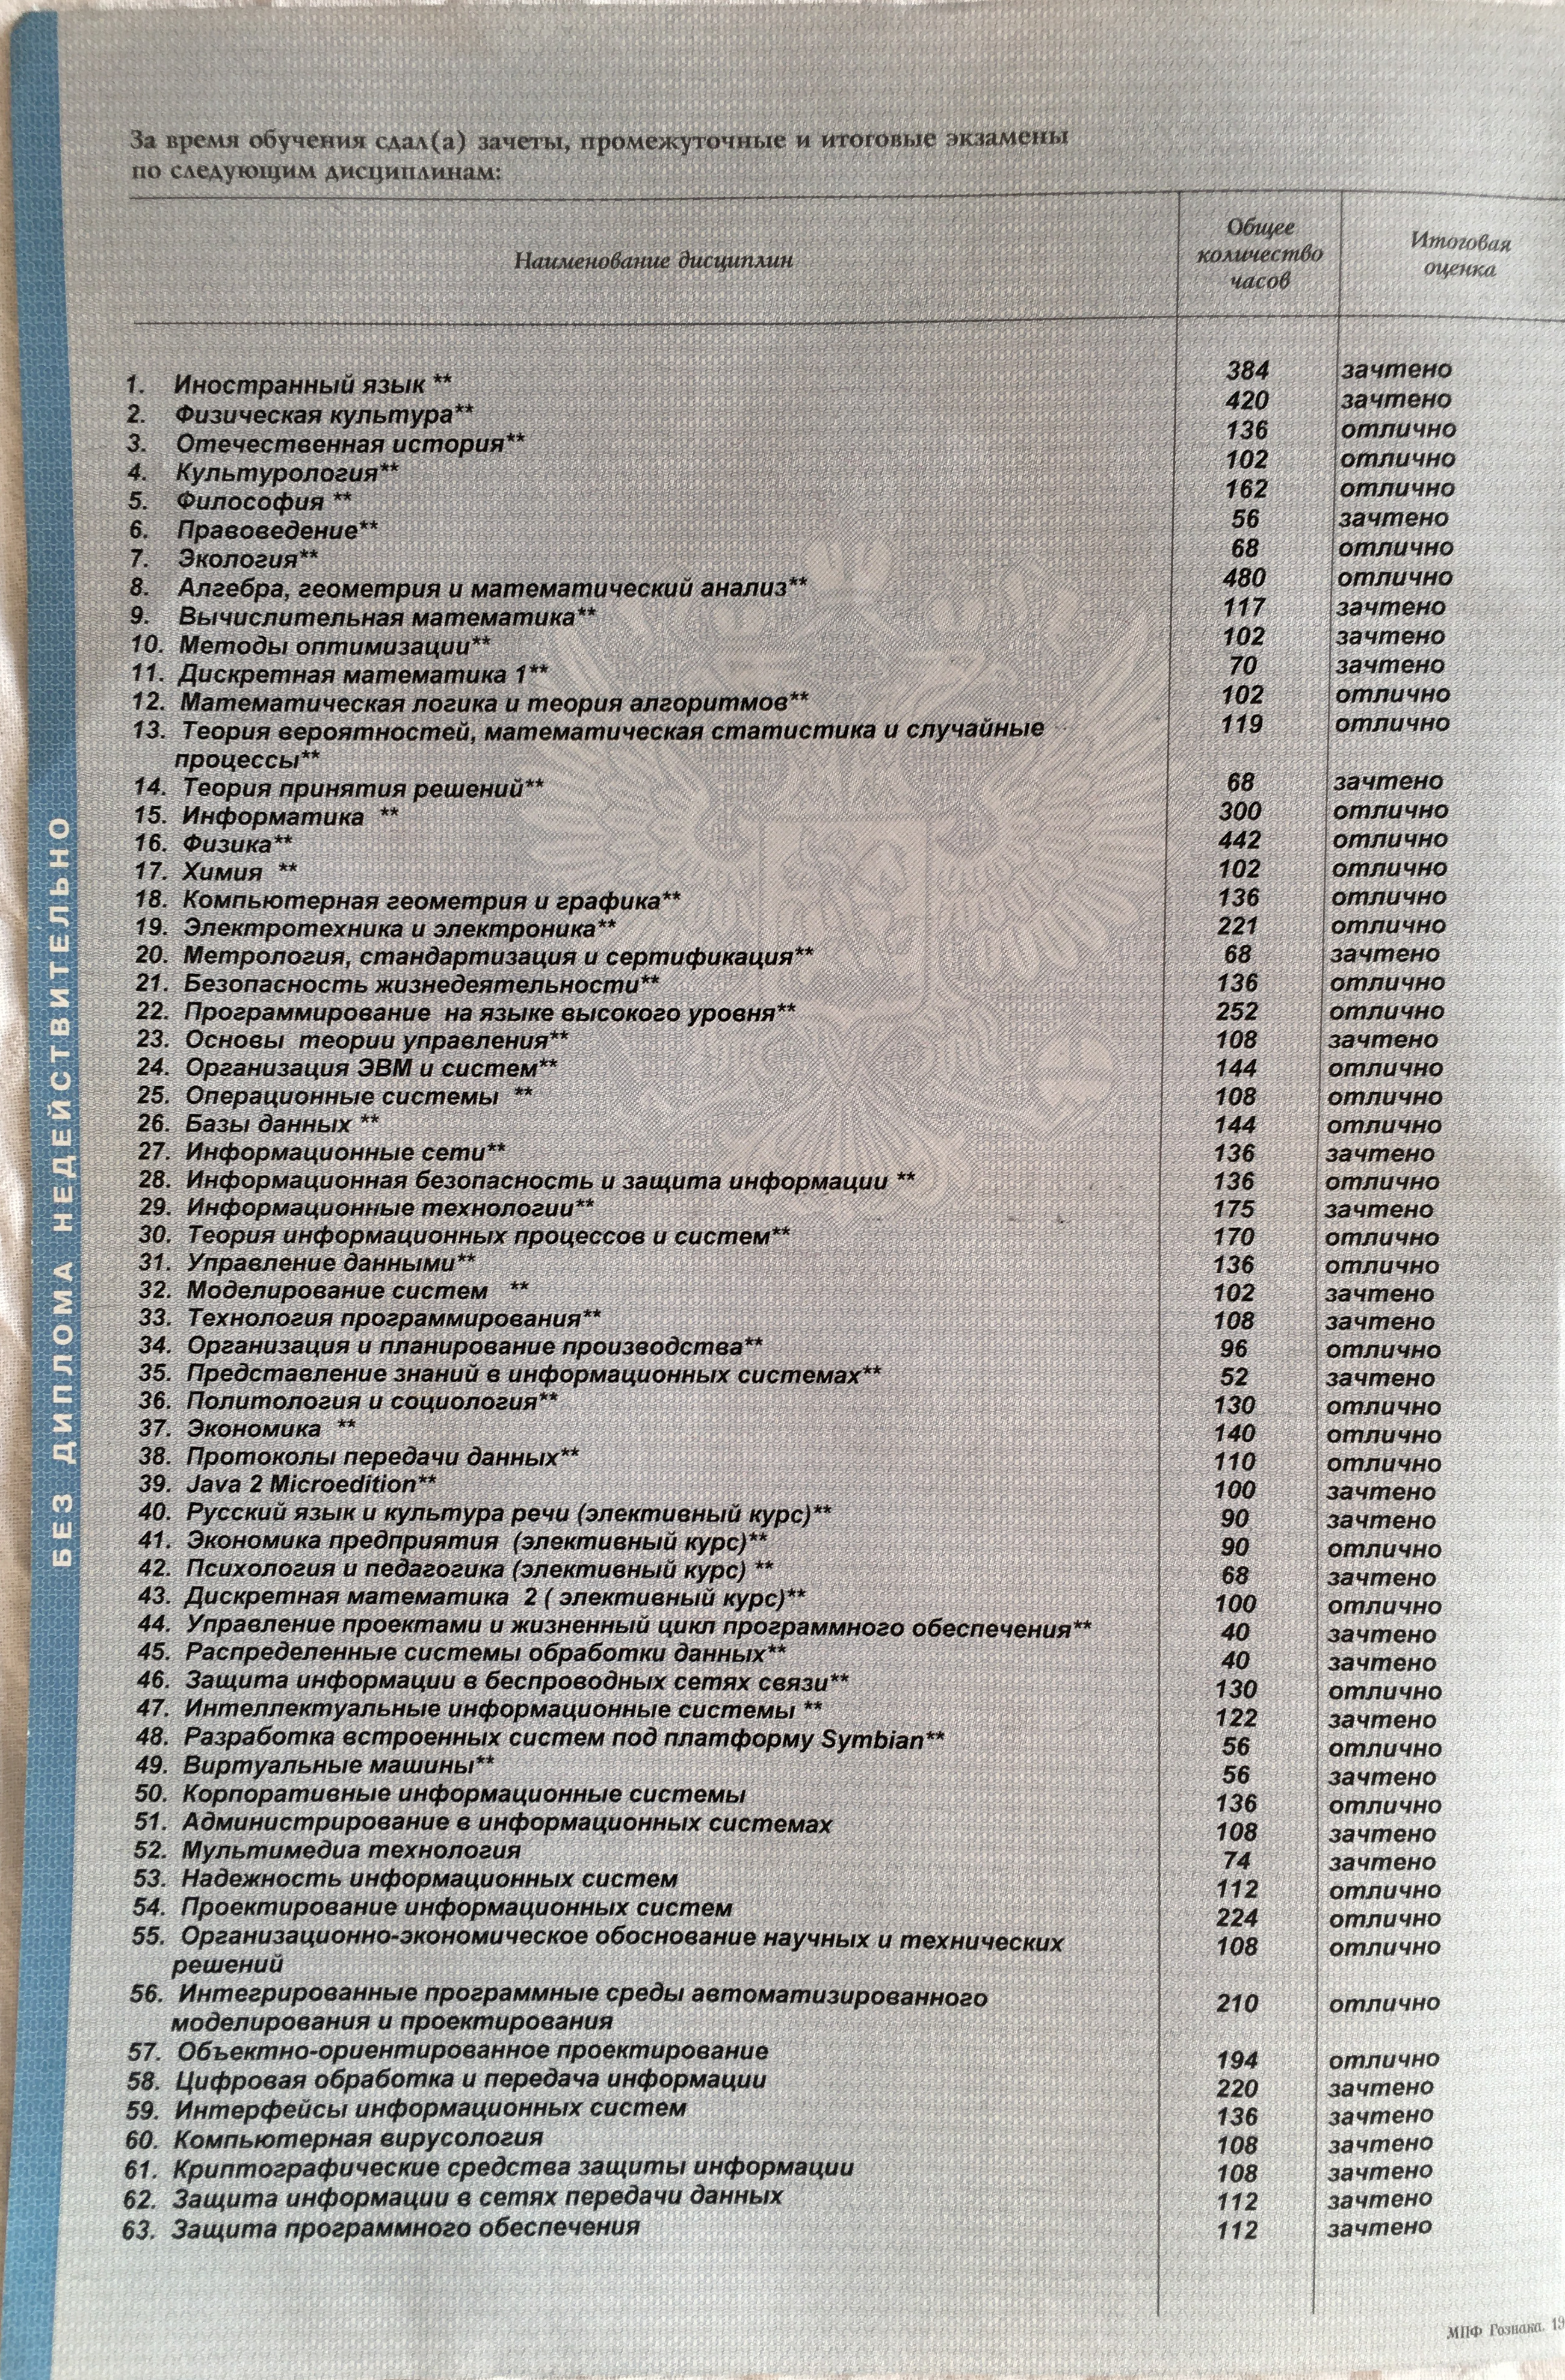
\includegraphics[width=38em]{appendix-2}
\end{center}
\pagebreak

\pagebreak
